\documentclass[10pt,twoside,openright,dvipdfmx]{jsbook}

%------------------------------%
% geometry
%------------------------------%

%\usepackage[pass,showframe]{geometry}
\usepackage[pass]{geometry}

%------------------------------%
% afterpage
%------------------------------%

\usepackage{afterpage}
\newcommand\blankpage{%
    \null
    \thispagestyle{empty}
    \addtocounter{page}{-1}
    \newpage
}

%------------------------------%
% mathtools
%------------------------------%

\usepackage{mathtools}

%------------------------------%
% makeidx
%------------------------------%

\usepackage{imakeidx}
\makeindex
\indexsetup{othercode={\thispagestyle{plain}}}

%------------------------------%
% fancyhdr
%------------------------------%

\usepackage{fancyhdr}

\pagestyle{fancy}
\fancyhf{}
\fancyhead[RO]{\leftmark}
\fancyhead[LE]{\rightmark}
\fancyfoot[LE,RO]{\thepage}
\setlength{\footskip}{12pt}

% TODO: apply beginning pages of chapter
\fancypagestyle{plain}{%
    \fancyhf{}
    \fancyfoot[LE,RO]{\thepage}
}

%------------------------------%
% color
%------------------------------%

\usepackage{color}
%http://www.biwako.shiga-u.ac.jp/sensei/kumazawa/tex/color.html
\definecolor{ikkonzome}{rgb}	{	0.9961	,	0.7569	,	0.7373	}
\definecolor{ishitake}{rgb}	{	0.9961	,	0.6941	,	0.7059	}
\definecolor{momo}{rgb}	        {	0.9961	,	0.6824	,	0.8039	}
\definecolor{kobai}{rgb}	{	0.9412	,	0.4235	,	0.5569	}
\definecolor{nakabeni}{rgb}	{	0.9451	,	0.2706	,	0.4941	}
\definecolor{sakura}{rgb}	{	0.9333	,	0.8353	,	0.8353	}
\definecolor{arazome}{rgb}	{	0.9725	,	0.7216	,	0.7843	}
\definecolor{usubeni}{rgb}	{	0.8471	,	0.4471	,	0.5451	}
\definecolor{hisame}{rgb}	{	0.7451	,	0.4039	,	0.4039	}
\definecolor{toki}{rgb}	        {	0.9569	,	0.6431	,	0.6353	}
\definecolor{sakuranezumi}{rgb}	{	0.6941	,	0.6039	,	0.6078	}
\definecolor{sango}	{rgb}	{	0.8471	,	0.4157	,	0.3725	}
\definecolor{akane}	{rgb}	{	0.7529	,	0.0118	,	0.3451	}
\definecolor{choshun}{rgb}	{	0.7490	,	0.5255	,	0.5255	}
\definecolor{karakurenai}{rgb}	{	0.7373	,	0.0118	,	0.2667	}
\definecolor{enji}{rgb}	        {	0.6275	,	0.0863	,	0.3176	}
\definecolor{keshiaka}{rgb}	{	0.6275	,	0.4275	,	0.4275	}
\definecolor{kokiake}{rgb}	{	0.5059	,	0.0706	,	0.2549	}
\definecolor{jinzamomi}{rgb}	{	0.9098	,	0.4549	,	0.4157	}
\definecolor{mizugaki}{rgb}	{	0.7294	,	0.5529	,	0.4784	}
\definecolor{umenezumi}{rgb}	{	0.5882	,	0.3922	,	0.3882	}
\definecolor{suoko}{rgb}        {	0.5843	,	0.2667	,	0.2431	}
\definecolor{akabeni}{rgb}	{	0.8039	,	0.0784	,	0.3725	}
\definecolor{shinshu}{rgb}	{	0.6431	,	0.0353	,	0.0000	}
\definecolor{azuki}{rgb}	{	0.5255	,	0.0235	,	0.0000	}
\definecolor{ginshu}{rgb}	{	0.7490	,	0.2824	,	0.0588	}
\definecolor{ebicha}{rgb}	{	0.4549	,	0.2706	,	0.2627	}
\definecolor{kuriume}{rgb}	{	0.5843	,	0.3804	,	0.4314	}
\definecolor{akebono}{rgb}	{	0.8902	,	0.5961	,	0.4941	}
\definecolor{hanezu}{rgb}	{	0.7882	,	0.5961	,	0.5373	}
\definecolor{sangoshu}{rgb}	{	0.8196	,	0.5059	,	0.4471	}
\definecolor{shozyohi}{rgb}	{	0.7686	,	0.0000	,	0.0000	}
\definecolor{shikancha}{rgb}	{	0.5569	,	0.3294	,	0.1882	}
\definecolor{kakishibu}{rgb}	{	0.6745	,	0.4078	,	0.3333	}
\definecolor{benikaba}{rgb}	{	0.7137	,	0.3373	,	0.2941	}
\definecolor{benitobi}{rgb}	{	0.6196	,	0.3176	,	0.2706	}
\definecolor{benihihada}{rgb}	{	0.5020	,	0.3137	,	0.2353	}
\definecolor{kurotobi}{rgb}	{	0.3176	,	0.2000	,	0.1490	}
\definecolor{benihi}{rgb}	{	0.8235	,	0.4745	,	0.1922	}
\definecolor{terigaki}{rgb}	{	0.8118	,	0.4627	,	0.1804	}
\definecolor{ake}{rgb}	        {	0.7804	,	0.3098	,	0.1725	}
\definecolor{edocha}{rgb}	{	0.6863	,	0.4353	,	0.2941	}
\definecolor{bengara}{rgb}	{	0.6392	,	0.1569	,	0.0196	}
\definecolor{hihada}{rgb}	{	0.5412	,	0.3412	,	0.2353	}
\definecolor{shishi}{rgb}	{	0.8549	,	0.6863	,	0.5961	}
\definecolor{araishu}{rgb}	{	0.9294	,	0.4902	,	0.4549	}
\definecolor{akago}{rgb}	{	0.8118	,	0.5765	,	0.4275	}
\definecolor{tokigaracha}{rgb}	{	0.7922	,	0.5255	,	0.3686	}
\definecolor{otan}{rgb}	        {	0.8157	,	0.4157	,	0.2235	}
\definecolor{komugi}{rgb}	{	0.8157	,	0.6549	,	0.5098	}
\definecolor{rakuda}{rgb}	{	0.6784	,	0.5255	,	0.4118	}
\definecolor{tsurubami}{rgb}	{	0.6275	,	0.4392	,	0.3961	}
\definecolor{ama}{rgb}	        {	0.7765	,	0.6902	,	0.5843	}
\definecolor{nikkei}{rgb}	{	0.7216	,	0.4667	,	0.3725	}
\definecolor{renga}{rgb}	{	0.6902	,	0.3765	,	0.3098	}
\definecolor{sohi}{rgb}   	{	0.8078	,	0.5098	,	0.2078	}
\definecolor{enshucha}{rgb}	{	0.6706	,	0.4275	,	0.1608	}
\definecolor{karacha}{rgb}	{	0.5765	,	0.4235	,	0.1490	}
\definecolor{kabacha}{rgb}	{	0.6353	,	0.3725	,	0.1569	}
\definecolor{sodenkaracha}{rgb}	{	0.5216	,	0.3490	,	0.1373	}
\definecolor{suzumecha}{rgb}	{	0.4745	,	0.3176	,	0.1255	}
\definecolor{kurikawacha}{rgb}	{	0.4078	,	0.2745	,	0.1098	}
\definecolor{momoshiocha}{rgb}	{	0.3490	,	0.2353	,	0.0902	}
\definecolor{tobi}{rgb}	        {	0.4353	,	0.3098	,	0.1412	}
\definecolor{kurumizome}{rgb}	{	0.6667	,	0.5333	,	0.3333	}
\definecolor{kaba}{rgb}	        {	0.8196	,	0.4588	,	0.1294	}
\definecolor{korosen}{rgb}	{	0.5059	,	0.3843	,	0.1608	}
\definecolor{kogecha}{rgb}	{	0.3333	,	0.2549	,	0.1098	}
\definecolor{kokikuchinashi}{rgb}	{	0.8078	,	0.5922	,	0.3490	}
\definecolor{araigaki}{rgb}	{	0.8157	,	0.5529	,	0.3176	}
\definecolor{taisha}{rgb}	{	0.6353	,	0.4196	,	0.2078	}
\definecolor{akashirotsurubami}{rgb}	{	0.8078	,	0.6118	,	0.4157	}
\definecolor{tonocha}{rgb}	{	0.5922	,	0.4039	,	0.2000	}
\definecolor{sencha}{rgb}	{	0.5255	,	0.3529	,	0.1490	}
\definecolor{sharegaki}{rgb}	{	0.8549	,	0.7098	,	0.4863	}
\definecolor{ko}{rgb}	        {	0.9529	,	0.8275	,	0.6627	}
\definecolor{usugaki}{rgb}	{	0.8627	,	0.7294	,	0.5294	}
\definecolor{koji}{rgb}	        {	0.8275	,	0.6039	,	0.2706	}
\definecolor{umezome}{rgb}	{	0.8667	,	0.7373	,	0.4235	}
\definecolor{beniukon}{rgb}	{	0.8549	,	0.5843	,	0.2549	}
\definecolor{chojicha}{rgb}	{	0.5569	,	0.4000	,	0.1098	}
\definecolor{kenpozome}{rgb}	{	0.3059	,	0.2667	,	0.0627	}
\definecolor{biwacha}{rgb}	{	0.7333	,	0.5294	,	0.1922	}
\definecolor{kohaku}{rgb}	{	0.8039	,	0.5961	,	0.2471	}
\definecolor{usuko}{rgb}	{	0.8745	,	0.7373	,	0.4824	}
\definecolor{kuchiba}{rgb}	{	0.8157	,	0.6157	,	0.3216	}
\definecolor{kincha}{rgb}	{	0.7725	,	0.4902	,	0.2000	}
\definecolor{chozizome}{rgb}	{	0.5686	,	0.3961	,	0.1608	}
\definecolor{kitsune}{rgb}	{	0.6392	,	0.4431	,	0.1804	}
\definecolor{hushizome}{rgb}	{	0.5804	,	0.4353	,	0.1608	}
\definecolor{kyara}{rgb}	{	0.4510	,	0.3373	,	0.1255	}
\definecolor{susutake}{rgb}	{	0.4588	,	0.3529	,	0.1176	}
\definecolor{shirocha}{rgb}	{	0.7529	,	0.6588	,	0.4118	}
\definecolor{odo}{rgb}	        {	0.7137	,	0.6039	,	0.3137	}
\definecolor{ginsusutake}{rgb}	{	0.5608	,	0.4745	,	0.2392	}
\definecolor{kigaracha}{rgb}	{	0.7490	,	0.6196	,	0.2745	}
\definecolor{kobicha}	{rgb}	{	0.5020	,	0.4118	,	0.1765	}
\definecolor{usuki}	{rgb}	{	0.8549	,	0.7804	,	0.4275	}
\definecolor{yamabuki}	{rgb}	{	0.9098	,	0.8000	,	0.2039	}
\definecolor{tamago}	{rgb}	{	0.8275	,	0.7412	,	0.3373	}
\definecolor{hajizome}	{rgb}	{	0.7412	,	0.6039	,	0.2431	}
\definecolor{yamabukicha}{rgb}	{	0.7059	,	0.5765	,	0.2275	}
\definecolor{kuwazome}	{rgb}	{	0.6471	,	0.5255	,	0.2118	}
\definecolor{namakabe}	{rgb}	{	0.5569	,	0.4549	,	0.1843	}
\definecolor{kuchinashi}{rgb}	{	0.8078	,	0.7333	,	0.3843	}
\definecolor{tomorokoshi}{rgb}	{	0.7804	,	0.7020	,	0.2941	}
\definecolor{shirotsurubami}{rgb}	{	0.8745	,	0.8235	,	0.5922	}
\definecolor{kitsurubami}{rgb}	{	0.6863	,	0.6039	,	0.2118	}
\definecolor{toou}	{rgb}	{	0.8353	,	0.7725	,	0.4235	}
\definecolor{hanaba}	{rgb}	{	0.8549	,	0.8000	,	0.4941	}
\definecolor{torinoko}	{rgb}	{	0.8431	,	0.8118	,	0.6902	}
\definecolor{ukon}	{rgb}	{	0.8039	,	0.7216	,	0.3059	}
\definecolor{kikuchiba}	{rgb}	{	0.7765	,	0.6667	,	0.2902	}
\definecolor{rikyushiracha}{rgb}{	0.6627	,	0.6471	,	0.4784	}
\definecolor{rikyucha}	{rgb}	{	0.5176	,	0.5176	,	0.2588	}
\definecolor{aku}	{rgb}	{	0.5294	,	0.5059	,	0.4039	}
\definecolor{higosusutake}{rgb}	{	0.4863	,	0.4510	,	0.3059	}
\definecolor{rokocha}	{rgb}	{	0.4157	,	0.4353	,	0.3686	}
\definecolor{mirucha}	{rgb}	{	0.4471	,	0.4471	,	0.3725	}
\definecolor{natane}	{rgb}	{	0.7216	,	0.6863	,	0.3882	}
\definecolor{kimirucha}	{rgb}	{	0.5373	,	0.5059	,	0.2549	}
\definecolor{uguisucha}	{rgb}	{	0.4118	,	0.3882	,	0.1961	}
\definecolor{nanohana}	{rgb}	{	0.9882	,	0.9882	,	0.3804	}
\definecolor{kariyasu}	{rgb}	{	0.8039	,	0.7686	,	0.3882	}
\definecolor{kihada}	{rgb}	{	0.9608	,	0.9137	,	0.2863	}
\definecolor{zoge}	{rgb}	{	0.8863	,	0.8235	,	0.7216	}
\definecolor{wara}	{rgb}	{	0.7882	,	0.7490	,	0.4706	}
\definecolor{macha}	{rgb}	{	0.6235	,	0.6392	,	0.4863	}
\definecolor{yamabato}	{rgb}	{	0.5137	,	0.5176	,	0.4000	}
\definecolor{mushikuri}	{rgb}	{	0.8196	,	0.8000	,	0.6118	}
\definecolor{aokuchiba}	{rgb}	{	0.6275	,	0.6392	,	0.3451	}
\definecolor{hiwacha}	{rgb}	{	0.6784	,	0.6863	,	0.4196	}
\definecolor{ominaeshi}	{rgb}	{	0.8745	,	0.8863	,	0.4039	}
\definecolor{wasabi}	{rgb}	{	0.5922	,	0.6824	,	0.5765	}
\definecolor{uguisu}	{rgb}	{	0.3333	,	0.4118	,	0.0627	}
\definecolor{hiwa}	{rgb}	{	0.7098	,	0.7216	,	0.2392	}
\definecolor{aoshirotsurubami}{rgb}	{	0.5961	,	0.6471	,	0.4471	}
\definecolor{yanagicha}	{rgb}	{	0.5373	,	0.5725	,	0.3529	}
\definecolor{rikancha}	{rgb}	{	0.3333	,	0.4196	,	0.2863	}
\definecolor{aikobicha}	{rgb}	{	0.2706	,	0.3412	,	0.2353	}
\definecolor{koke}	{rgb}	{	0.4941	,	0.5686	,	0.3922	}
\definecolor{miru}	{rgb}	{	0.1529	,	0.3216	,	0.1843	}
\definecolor{sensai}	{rgb}	{	0.1373	,	0.2863	,	0.1608	}
\definecolor{baiko}	{rgb}	{	0.5529	,	0.6157	,	0.3922	}
\definecolor{iwai}	{rgb}	{	0.3059	,	0.4118	,	0.2784	}
\definecolor{hiwamoegi}	{rgb}	{	0.4431	,	0.6824	,	0.2431	}
\definecolor{yanagisusutake}{rgb}	{	0.2039	,	0.3333	,	0.1255	}
\definecolor{urayanagi}	{rgb}	{	0.5843	,	0.6824	,	0.2431	}
\definecolor{usumoegi}	{rgb}	{	0.4824	,	0.6706	,	0.2275	}
\definecolor{yanagizome}{rgb}	{	0.4353	,	0.6000	,	0.2078	}
\definecolor{moegi}	{rgb}	{	0.3020	,	0.5961	,	0.1882	}
\definecolor{aoni}	{rgb}	{	0.1216	,	0.4196	,	0.2431	}
\definecolor{matsuba}	{rgb}	{	0.1098	,	0.3686	,	0.2118	}
\definecolor{usuao}	{rgb}	{	0.5529	,	0.7059	,	0.6118	}
\definecolor{wakatake}	{rgb}	{	0.3843	,	0.6824	,	0.5059	}
\definecolor{yanaginezumi}{rgb}	{	0.5020	,	0.6078	,	0.5490	}
\definecolor{oitake}	{rgb}	{	0.4157	,	0.5412	,	0.4392	}
\definecolor{sensaimidori}{rgb}	{	0.2549	,	0.3882	,	0.2627	}
\definecolor{midori}	{rgb}	{	0.0000	,	0.4824	,	0.0000	}
\definecolor{byakuroku}	{rgb}	{	0.6078	,	0.7333	,	0.6196	}
\definecolor{sabiseiji}	{rgb}	{	0.5333	,	0.6588	,	0.5804	}
\definecolor{rokusho}	{rgb}	{	0.3373	,	0.6039	,	0.4039	}
\definecolor{tokusa}	{rgb}	{	0.2549	,	0.4706	,	0.3922	}
\definecolor{onandocha}	{rgb}	{	0.2039	,	0.3725	,	0.3098	}
\definecolor{aotake}	{rgb}	{	0.1412	,	0.5176	,	0.4353	}
\definecolor{rikyunezumi}{rgb}	{	0.4157	,	0.5686	,	0.5490	}
\definecolor{birodo}	{rgb}	{	0.1059	,	0.4275	,	0.3608	}
\definecolor{mishiao}	{rgb}	{	0.1098	,	0.4588	,	0.3882	}
\definecolor{aimirucha}	{rgb}	{	0.2510	,	0.4000	,	0.3608	}
\definecolor{tonotya}	{rgb}	{	0.3059	,	0.4941	,	0.4392	}
\definecolor{mizuasagi}	{rgb}	{	0.1569	,	0.6745	,	0.6745	}
\definecolor{seji}	{rgb}	{	0.4745	,	0.6588	,	0.5922	}
\definecolor{seheki}	{rgb}	{	0.0588	,	0.5569	,	0.4824	}
\definecolor{sabitetsu}	{rgb}	{	0.0392	,	0.3294	,	0.2784	}
\definecolor{tetsu}	{rgb}	{	0.0627	,	0.3961	,	0.3961	}
\definecolor{omeshicha}	{rgb}	{	0.0667	,	0.4667	,	0.4667	}
\definecolor{korainando}{rgb}	{	0.0588	,	0.3922	,	0.0392	}
\definecolor{minatonezumi}{rgb}	{	0.4549	,	0.6000	,	0.6118	}
\definecolor{aonibi}	{rgb}	{	0.1804	,	0.3725	,	0.3882	}
\definecolor{tetsuonando}{rgb}	{	0.1961	,	0.4118	,	0.4275	}
\definecolor{mizu}	{rgb}	{	0.5451	,	0.7412	,	0.7608	}
\definecolor{sabiasagi}	{rgb}	{	0.4510	,	0.6000	,	0.6000	}
\definecolor{kamenozoki}{rgb}	{	0.7098	,	0.9020	,	0.8902	}
\definecolor{asagi}	{rgb}	{	0.3020	,	0.6784	,	0.7098	}
\definecolor{shinbashi}	{rgb}	{	0.0000	,	0.6000	,	0.6353	}
\definecolor{sabionando}{rgb}	{	0.2392	,	0.3961	,	0.3843	}
\definecolor{ainezumi}	{rgb}	{	0.2235	,	0.4000	,	0.3843	}
\definecolor{ai}	{rgb}	{	0.2039	,	0.3765	,	0.4314	}
\definecolor{onando}	{rgb}	{	0.1843	,	0.3686	,	0.4000	}
\definecolor{hanaasagi}	{rgb}	{	0.2000	,	0.6196	,	0.7098	}
\definecolor{chigusa}	{rgb}	{	0.1922	,	0.5725	,	0.6745	}
\definecolor{masuhana}	{rgb}	{	0.1569	,	0.4667	,	0.5569	}
\definecolor{hanada}	{rgb}	{	0.0039	,	0.4275	,	0.5373	}
\definecolor{noshimehana}{rgb}	{	0.1412	,	0.4235	,	0.5098	}
\definecolor{omeshionando}{rgb}	{	0.1176	,	0.3529	,	0.4235	}
\definecolor{sora}	{rgb}	{	0.1451	,	0.7216	,	0.8039	}
\definecolor{konpeki}	{rgb}	{	0.0902	,	0.5098	,	0.7333	}
\definecolor{kurotsurubami}{rgb}{	0.0627	,	0.3137	,	0.3451	}
\definecolor{gunjo}	{rgb}	{	0.5098	,	0.7882	,	0.9098	}
\definecolor{kon}	{rgb}	{	0.0000	,	0.2000	,	0.4000	}
\definecolor{kachi}	{rgb}	{	0.0000	,	0.1765	,	0.3490	}
\definecolor{ruri}	{rgb}	{	0.0078	,	0.3922	,	0.6510	}
\definecolor{konjo}	{rgb}	{	0.0039	,	0.3137	,	0.5216	}
\definecolor{rurikon}	{rgb}	{	0.0000	,	0.3020	,	0.5020	}
\definecolor{benimidori}{rgb}	{	0.3373	,	0.4588	,	0.6784	}
\definecolor{konkikyo}	{rgb}	{	0.0039	,	0.0667	,	0.4275	}
\definecolor{hujinezumi}{rgb}	{	0.3216	,	0.3686	,	0.6118	}
\definecolor{benikakehana}{rgb}	{	0.2275	,	0.2471	,	0.5882	}
\definecolor{hujiiro}	{rgb}	{	0.4706	,	0.4863	,	0.7059	}
\definecolor{hutaai}	{rgb}	{	0.3137	,	0.3333	,	0.5608	}
\definecolor{hujimurasaki}{rgb}	{	0.4157	,	0.3333	,	0.5686	}
\definecolor{kikyo}	{rgb}	{	0.3529	,	0.3216	,	0.5725	}
\definecolor{shion}	{rgb}	{	0.5137	,	0.4196	,	0.6784	}
\definecolor{messhi}	{rgb}	{	0.2196	,	0.1765	,	0.3098	}
\definecolor{shikon}	{rgb}	{	0.2510	,	0.1961	,	0.3529	}
\definecolor{kokimurasaki}{rgb}	{	0.3098	,	0.2000	,	0.3765	}
\definecolor{usu}	{rgb}	{	0.7294	,	0.6353	,	0.7843	}
\definecolor{hashita}	{rgb}	{	0.6000	,	0.4549	,	0.6706	}
\definecolor{rindo}	{rgb}	{	0.5922	,	0.5137	,	0.7529	}
\definecolor{sumire}	{rgb}	{	0.3882	,	0.2157	,	0.5922	}
\definecolor{nasukon}	{rgb}	{	0.3216	,	0.2235	,	0.4353	}
\definecolor{murasaki}	{rgb}	{	0.3137	,	0.1765	,	0.4824	}
\definecolor{kurobeni}	{rgb}	{	0.2353	,	0.1294	,	0.3059	}
\definecolor{ayame}	{rgb}	{	0.4275	,	0.1569	,	0.5098	}
\definecolor{benihuji}	{rgb}	{	0.6824	,	0.5333	,	0.6667	}
\definecolor{edomurasaki}{rgb}	{	0.3961	,	0.1529	,	0.4392	}
\definecolor{kodaimurasaki}{rgb}{	0.4353	,	0.2863	,	0.4627	}
\definecolor{shikon}{rgb}       {	0.4118	,	0.2549	,	0.3765	}
\definecolor{hatobanezumi}{rgb}	{	0.4235	,	0.3804	,	0.4392	}
\definecolor{budonezumi}{rgb}	{	0.3412	,	0.2196	,	0.3529	}
\definecolor{ebizome}	{rgb}	{	0.4000	,	0.2235	,	0.3882	}
\definecolor{hujisusutake}{rgb}	{	0.2549	,	0.0824	,	0.2471	}
\definecolor{usuebi}	{rgb}	{	0.6549	,	0.4392	,	0.6039	}
\definecolor{botan}	{rgb}	{	0.6706	,	0.0392	,	0.4353	}
\definecolor{umemurasaki}{rgb}	{	0.6667	,	0.3922	,	0.5176	}
\definecolor{nisemurasaki}{rgb}	{	0.3686	,	0.0000	,	0.3216	}
\definecolor{murasakitobi}{rgb}	{	0.3922	,	0.3255	,	0.3529	}
\definecolor{ususuo}{rgb}	{	0.7569	,	0.4000	,	0.5412	}
\definecolor{suo}{rgb}	        {	0.6941	,	0.0627	,	0.4157	}
\definecolor{kuwanomi}{rgb}	{	0.4196	,	0.0549	,	0.2745	}
\definecolor{nibi}{rgb}	        {	0.4549	,	0.4235	,	0.3961	}
\definecolor{benikeshi}{rgb}	{	0.4118	,	0.3804	,	0.3843	}
\definecolor{shironeri}{rgb}	{	0.9843	,	0.9843	,	0.9843	}
\definecolor{shironezumi}{rgb}	{	0.6471	,	0.6588	,	0.6627	}
\definecolor{ginnezumi}{rgb}	{	0.5255	,	0.5490	,	0.5922	}
\definecolor{sunezumi}{rgb}	{	0.4275	,	0.4392	,	0.4392	}
\definecolor{dobunezumi}{rgb}	{	0.2863	,	0.2941	,	0.2941	}
\definecolor{aisumicha}{rgb}	{	0.2078	,	0.2196	,	0.2510	}
\definecolor{binrojizome}{rgb}	{	0.2118	,	0.0824	,	0.0706	}
\definecolor{sumizome}{rgb}	{	0.2706	,	0.2706	,	0.2706	}


%------------------------------%
% graphicx
%------------------------------%

\usepackage{graphicx}

%------------------------------%
% listings
%------------------------------%

\usepackage{listings,jlisting}
\lstdefinelanguage{swift}{
    sensitive=true,
    alsoletter={\#},
    keywords=[1]{associatedtype,class,deinit,enum,extension,fileprivate,func,import,init,inout,internal,let,open,operator,private,protocol,public,static,struct,subscript,typealias,var,break,case,continue,default,defer,do,else,fallthrough,for,guard,if,in,repeat,return,switch,where,while,as,Any,catch,false,is,nil,rethrows,super,self,Self,throw,throws,true,try,\_,associativity,convenience,dynamic,didSet,final,get,infix,indirect,lazy,left,mutating,none,nonmutating,optional,override,postfix,precedence,prefix,Protocol,required,right,set,Type,unowned,weak,willSet},
    keywords=[2]{\#available,\#colorLiteral,\#column,\#else,\#elseif,\#endif,\#file,\#fileLiteral,\#function,\#if,\#imageLiteral,\#line,\#selector,\#sourceLocation,@autoclosure},
    numbers=left,
    numberstyle=\scriptsize,
    stepnumber=1,
    numbersep=8pt,
    showstringspaces=false,
    breaklines=true,
    morecomment=[l]{//},
    morecomment=[s]{/*}{*/},
    keywordstyle=[1]\color{konpeki},
    keywordstyle=[2]\color{rindo},
    commentstyle=\color{usumoegi},
    stringstyle=\color{enji},
    morestring=[b]",%"
}

\renewcommand{\lstlistingname}{プログラム}
\lstset{language=swift,
    basicstyle=\ttfamily\scriptsize,
    commentstyle=\textit,
    classoffset=1,
    keywordstyle=\bfseries,
    frame=tRBl,
    framesep=5pt,
    showstringspaces=false,
    numbers=left,
    stepnumber=1,
    numberstyle=\tiny,
    tabsize=2
}



%------------------------------%
% box
%------------------------------%

\usepackage{ascmac,fancybox}

%------------------------------%
% appendix
%------------------------------%

\usepackage[toc,page]{appendix}

\makeatletter
\AtBeginEnvironment{appendices}{%
  \clearpage%
  \fancypagestyle{plain}{%
    \fancyhf{}%
    \renewcommand{\headrulewidth}{0pt}
  }
  \thispagestyle{plain}
}

%------------------------------%
% biblatex
%------------------------------%

\usepackage[style=numeric,backend=biber,defernumbers=true]{biblatex}
\addbibresource{bibliographies/iosdc.bib}
\addbibresource{bibliographies/apple.bib}
\addbibresource{bibliographies/other.bib}

%------------------------------%
% accented letters
%------------------------------%

\usepackage[utf8]{inputenc}

%------------------------------%
% development
%------------------------------%

\usepackage{lipsum}
\usepackage{layout}

%------------------------------%
% title
%------------------------------%

\usepackage{authblk}

\title{%
    iOSDC 2018 Draft \\
    \large for \href{https://fortee.jp/iosdc-japan-2018/proposal/8e9e8e22-8ff1-4381-813a-347475c2606f}{フォントと組版の30分入門}}
\author[$\dagger$]{しもとりしぐれ}
\affil[$\dagger$]{@S\_Shimotori}
\date{\today}

%------------------------------%
% hyperref
%------------------------------%

\usepackage[colorlinks]{hyperref}

\hypersetup{
    urlcolor=hujinezumi,
    citecolor=sora,
    linkcolor=black
}

\usepackage[normalem]{ulem}

\makeatletter
\begingroup
    \catcode`\$=6
    \catcode`\#=12
    \gdef\href@split$1#$2#$3\\$4{
        \hyper@@link{$1}{$2}{\uline{$4}}
        \endgroup
    }%
\endgroup

%------------------------------%
% document
%------------------------------%

\begin{document}

\pagenumbering{Alph}
\newgeometry{hmarginratio=1:1}
\maketitle
\restoregeometry

\afterpage{\blankpage}

\pagenumbering{roman}

\tableofcontents
\thispagestyle{plain}

\chapter*{はしがき}
\thispagestyle{plain}
\addcontentsline{toc}{chapter}{はしがき}
iOSDC 2018\cite{iosdc.jp:2018}では「iOSエンジニアに聞いて欲しいトーク(30分)」という枠が追加されました.

\begin{quote}
トークのテーマは必ずしもiOS関連の話である必要はありません。iOSエンジニアが聞いて面白ければ何でもアリです!
\end{quote}

\noindent とのことです\cite{fortee.jp:iosdc-japan-2018/speaker/proposal/cfp}.そこで,「フォントと組版の30分入門」とタイトルをつけて次の説明文とともにプロポーザルを出しました\cite{fortee.jp:iosdc-japan-2018/proposal/8e9e8e22-8ff1-4381-813a-347475c2606f}.要するにニッチな方向に攻めました.

\begin{quote}
フォントや組版について気にしたことはありますか? \\
奥深く興味深い世界ですが、そのぶん難しい用語や規則がたくさん。間違えるとこわーい人にツッコミを入れられてしまうかも! \\
本セッションでは、日頃TextKitと親しくしている皆様、技術同人誌に興味のある皆様を対象に、基礎とちょっとした雑学を学びます。
\end{quote}

\noindent 言語実装でもハードウェアでもネットワークでもサーバサイドでもない話題です.怖くなったので強引にTextKitという言葉を出してごまかしています.また,発表の意義を高めるために技術同人誌という言葉も出しました.Twitterには

\begin{quote}
\noindent フォントと組版の30分入門 by S\_Shimotori \textbar プロポーザル \textbar iOSDC Japan 2018 - \href{https://t.co/DZDIy0aFCd}{https://fortee.jp/} \href{https://t.co/zvSrclhYoT}{https://fortee.jp/iosdc-japan-20 \ldots}せっかくのiOSDCなので、WWDCのTextKitのセッションに対抗してDTP方面の話をしたいです!よろしくお願いします!!
\end{quote}

\noindent と投稿して宣伝しました\cite{twitter.com:S_Shimotori_pub/status/1008257832863428609}.せっかくのiOSDCですから,iOSのコアな話をするのが王道でしょうが,そのようなネタは結局最後まで思い浮かばなかったので応募しませんでした.

こうした経緯により,皆様の応援をもって「フォントと組版の30分入門」は無事採択となりました.「iOSエンジニアに聞いて欲しいトーク(30分)」枠かつニッチ狙いですので,iOSで縦書きを試みるような実用的な話は行わないつもりです.よろしくお願いします.

\begin{flushright}
2018年7月14日 \\
しもとりしぐれ
\end{flushright}



\cleardoublepage

%------------------------------%

\pagenumbering{arabic}

\newgeometry{hmarginratio=1:1}
\part{基礎編(仮)}
\restoregeometry

\chapter{用語解説(仮)}
あとで消す

\begin{figure}
    \begin{center}
        
\includegraphics[width=10cm]{images/typography_terms_apple.png}
    \end{center}
    \caption{\cite{developer.apple.com:library/archive/documentation/StringsTextFonts/Conceptual/TextAndWebiPhoneOS/Introduction/Introduction.html}}
\end{figure}

\begin{figure}
    \begin{center}
        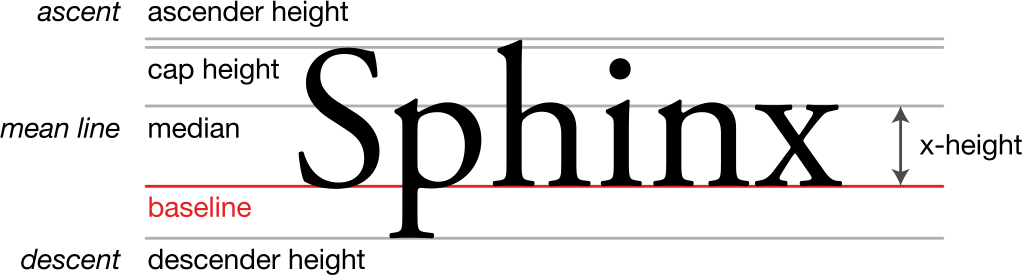
\includegraphics[width=10cm]{images/typography_terms_wikipedia.png}
    \end{center}
    \caption{\cite{en.wikipedia.org/wiki/File:Typography_Line_Terms.svg}}
\end{figure}



\newgeometry{hmarginratio=1:1}
\part{internationalization(仮)}\label{part:internationalization}
\restoregeometry

\chapter{色々な言語(仮)}\label{chapter:internationalization/languages}
\thispagestyle{plain}
本章では,iOSで文字列の縦書きを試みる.iOSでの描画には通常UIKitを用いる.UIKitではラベルの描画のために{\sf UILabel}クラスが用意されている.

\begin{lstlisting}[language=swift,caption=Plainモードの{\sf UILabel},label=lst:ios/vertical/uilabel_and_string]
let label = UILabel()
label.backgroundColor = .white
label.textColor = .gray
label.text = "フォントと組版の30分入門"
label.sizeToFit()
\end{lstlisting}

\begin{lstlisting}[language=swift,caption=Attributedモードの{\sf UILabel},label=lst:ios/vertical/uilabel_and_nsattributedstring]
let label = UILabel()
let attributed = NSMutableAttributedString(string: "フォントと組版の30分入門")
attributed.addAttribute(.foregroundColor, value: UIColor.gray, range: NSRange(location: 0, length: 7))
attributed.addAttribute(.backgroundColor, value: UIColor.white, range: NSRange(location: 0, length: 13))
label.attributedText = attributed
label.sizeToFit()
\end{lstlisting}

プログラム\ref{lst:ios/vertical/uilabel_and_string}とプログラム\ref{lst:ios/vertical/uilabel_and_nsattributedstring}は{\sf UILabel}の使用例である.{\sf UILabel}は,{\sf text}プロパティに{\sf String}({\sf NSString})を渡すとPlainモードに,{\sf attributedText}プロパティに{\sf NSAttributedString}を渡すとAttributedモードになる\cite{developer.apple.com:documentation/uikit/uilabel}.
{\sf NSAttributedString}の属性キー{\sf NSAttributedString.Key}には文字列の方向を定める{\sf verticalGlyphForm}があるが,iOSでは常に横書きとされるため値を設定しても縦書きにならない\footnote{{\sf verticalGlyphForm}そのものはiOS 6.0以降で使える.iOS6って2012年なんだけどなぁ.}\cite{developer.apple.com:documentation/foundation/nsattributedstring/key/1528658-verticalglyphform}.



\newgeometry{hmarginratio=1:1}
\part{iOS}\label{part:ios}
\restoregeometry

\chapter{iOSにおけるRTLレイアウト}\label{chapter:ios/rtl}
\thispagestyle{plain}
本章では,iOSで文字列の縦書きを試みる.iOSでの描画には通常UIKitを用いる.UIKitではラベルの描画のために{\sf UILabel}クラスが用意されている.

\begin{lstlisting}[language=swift,caption=Plainモードの{\sf UILabel},label=lst:ios/vertical/uilabel_and_string]
let label = UILabel()
label.backgroundColor = .white
label.textColor = .gray
label.text = "フォントと組版の30分入門"
label.sizeToFit()
\end{lstlisting}

\begin{lstlisting}[language=swift,caption=Attributedモードの{\sf UILabel},label=lst:ios/vertical/uilabel_and_nsattributedstring]
let label = UILabel()
let attributed = NSMutableAttributedString(string: "フォントと組版の30分入門")
attributed.addAttribute(.foregroundColor, value: UIColor.gray, range: NSRange(location: 0, length: 7))
attributed.addAttribute(.backgroundColor, value: UIColor.white, range: NSRange(location: 0, length: 13))
label.attributedText = attributed
label.sizeToFit()
\end{lstlisting}

プログラム\ref{lst:ios/vertical/uilabel_and_string}とプログラム\ref{lst:ios/vertical/uilabel_and_nsattributedstring}は{\sf UILabel}の使用例である.{\sf UILabel}は,{\sf text}プロパティに{\sf String}({\sf NSString})を渡すとPlainモードに,{\sf attributedText}プロパティに{\sf NSAttributedString}を渡すとAttributedモードになる\cite{developer.apple.com:documentation/uikit/uilabel}.
{\sf NSAttributedString}の属性キー{\sf NSAttributedString.Key}には文字列の方向を定める{\sf verticalGlyphForm}があるが,iOSでは常に横書きとされるため値を設定しても縦書きにならない\footnote{{\sf verticalGlyphForm}そのものはiOS 6.0以降で使える.iOS6って2012年なんだけどなぁ.}\cite{developer.apple.com:documentation/foundation/nsattributedstring/key/1528658-verticalglyphform}.



\chapter{TextKit解説(仮)}\label{chapter:ios/textKit}
\thispagestyle{plain}
本章では,iOSで文字列の縦書きを試みる.iOSでの描画には通常UIKitを用いる.UIKitではラベルの描画のために{\sf UILabel}クラスが用意されている.

\begin{lstlisting}[language=swift,caption=Plainモードの{\sf UILabel},label=lst:ios/vertical/uilabel_and_string]
let label = UILabel()
label.backgroundColor = .white
label.textColor = .gray
label.text = "フォントと組版の30分入門"
label.sizeToFit()
\end{lstlisting}

\begin{lstlisting}[language=swift,caption=Attributedモードの{\sf UILabel},label=lst:ios/vertical/uilabel_and_nsattributedstring]
let label = UILabel()
let attributed = NSMutableAttributedString(string: "フォントと組版の30分入門")
attributed.addAttribute(.foregroundColor, value: UIColor.gray, range: NSRange(location: 0, length: 7))
attributed.addAttribute(.backgroundColor, value: UIColor.white, range: NSRange(location: 0, length: 13))
label.attributedText = attributed
label.sizeToFit()
\end{lstlisting}

プログラム\ref{lst:ios/vertical/uilabel_and_string}とプログラム\ref{lst:ios/vertical/uilabel_and_nsattributedstring}は{\sf UILabel}の使用例である.{\sf UILabel}は,{\sf text}プロパティに{\sf String}({\sf NSString})を渡すとPlainモードに,{\sf attributedText}プロパティに{\sf NSAttributedString}を渡すとAttributedモードになる\cite{developer.apple.com:documentation/uikit/uilabel}.
{\sf NSAttributedString}の属性キー{\sf NSAttributedString.Key}には文字列の方向を定める{\sf verticalGlyphForm}があるが,iOSでは常に横書きとされるため値を設定しても縦書きにならない\footnote{{\sf verticalGlyphForm}そのものはiOS 6.0以降で使える.iOS6って2012年なんだけどなぁ.}\cite{developer.apple.com:documentation/foundation/nsattributedstring/key/1528658-verticalglyphform}.



\chapter{iOSで縦書きを試みる(仮)}\label{chapter:ios/vertical}
\thispagestyle{plain}
本章では,iOSで文字列の縦書きを試みる.iOSでの描画には通常UIKitを用いる.UIKitではラベルの描画のために{\sf UILabel}クラスが用意されている.

\begin{lstlisting}[language=swift,caption=Plainモードの{\sf UILabel},label=lst:ios/vertical/uilabel_and_string]
let label = UILabel()
label.backgroundColor = .white
label.textColor = .gray
label.text = "フォントと組版の30分入門"
label.sizeToFit()
\end{lstlisting}

\begin{lstlisting}[language=swift,caption=Attributedモードの{\sf UILabel},label=lst:ios/vertical/uilabel_and_nsattributedstring]
let label = UILabel()
let attributed = NSMutableAttributedString(string: "フォントと組版の30分入門")
attributed.addAttribute(.foregroundColor, value: UIColor.gray, range: NSRange(location: 0, length: 7))
attributed.addAttribute(.backgroundColor, value: UIColor.white, range: NSRange(location: 0, length: 13))
label.attributedText = attributed
label.sizeToFit()
\end{lstlisting}

プログラム\ref{lst:ios/vertical/uilabel_and_string}とプログラム\ref{lst:ios/vertical/uilabel_and_nsattributedstring}は{\sf UILabel}の使用例である.{\sf UILabel}は,{\sf text}プロパティに{\sf String}({\sf NSString})を渡すとPlainモードに,{\sf attributedText}プロパティに{\sf NSAttributedString}を渡すとAttributedモードになる\cite{developer.apple.com:documentation/uikit/uilabel}.
{\sf NSAttributedString}の属性キー{\sf NSAttributedString.Key}には文字列の方向を定める{\sf verticalGlyphForm}があるが,iOSでは常に横書きとされるため値を設定しても縦書きにならない\footnote{{\sf verticalGlyphForm}そのものはiOS 6.0以降で使える.iOS6って2012年なんだけどなぁ.}\cite{developer.apple.com:documentation/foundation/nsattributedstring/key/1528658-verticalglyphform}.


\section{{\sf UILabel}幅の縮小による縦書き}\label{chapter:ios/vertical/numberOfLines}
最も簡単に縦書きにする方法は,{\sf UILabel}の幅をなるべく小さくすることで1文字ずつ改行させる方法である(プログラム\ref{lst:ios/vertical/uiLabelWidth/example}).

\begin{lstlisting}[language=swift,caption={\sf UILabel}の幅を縮小することによる縦書きの実現,label=lst:ios/vertical/uiLabelWidth/example]
let label = UILabel()
label.text = "30 minutes Introduction to Font and Typesetting"
label.font = UIFont(name: "Courier", size: 17)
label.numberOfLines = 0
label.frame = CGRect(x: 0, y: 0, width: 17, height: 500)
\end{lstlisting}

システムフォントのSan Francisco\footnote{正確にはSan Francisco Pro DisplayもしくはSan Francisco Pro Text.20pt以上でDisplayに,20pt未満でTextになる\cite{developer.apple.com:design/human-interface-guidelines/ios/visual-design/typography/}.}は等幅ではないため,Courierなどの等幅フォントにすることである程度綺麗に見せることができる.いずれにせよ,全角文字と半角文字が混ざった文字列や拗音は正しい位置に表示されない.



\newgeometry{hmarginratio=1:1}
\part{パート}\label{part:draft}
\restoregeometry

\chapter{チャプター}\label{chapter:draft}
\thispagestyle{plain}
チャプター

%------------------------------%

\newgeometry{hmarginratio=1:1}
\begin{appendices}
\restoregeometry
\chapter{用語集}
% TODO: fix
\thispagestyle{fancy}
用語(あとで消す)

モリサワとW3C\cite{www.w3.org:TR/2011/WD-jlreq-20111129/ja/}あたりから引用中.

\begin{description}
    \item[Advancement]
    \item[Alignment] alignmentとdirectionalityは異なるものを指すので注意\cite{developer.apple.com:videos/play/wwdc2016/232/}.
    \item[Ascent]
    \item[Baseline(並び線)]
    \item[base writing direction] 最初に登場したstrong characterで決定される\cite{developer.apple.com:videos/play/wwdc2016/232/}\cite{unicode.org:reports/tr9/}.
    \item[bidirectional algorithm(双方向アルゴリズム)] bidirectional textを扱うためのアルゴリズム\cite{www.w3.org:International/articles/inline-bidi-markup/uba-basics}.bidi algorithmとも.このアルゴリズムによる脆弱性が見つかったことがある\cite{jvndb.jvn.jp:ja/contents/2010/JVNDB-2010-002420.html}.
    \item[bidirectional text(双方向テキスト)] 左横書き(LTR)と右横書き(RTL)が混在するテキストのこと\cite{www.w3.org:International/articles/inline-bidi-markup/uba-basics}.bidiとも.
    \item[block direction(行送り方向)]
    \item[bold(太字)]
    \item[Boldface]
    \item[Bounding rectangle]
    \item[break (a line)(分割)]
    \item[Cap height]
    \item[centering(中央そろえ)]
    \item[character advance(字幅)]
    \item[character frame(外枠)]
    \item[characters not starting line(行頭禁則文字)]
    \item[CJK] 中国日本韓国,特に中国語・日本語・韓国語のこと.UnicodeのブロックにもCJKが散見される\cite{unicode.org:Public/UNIDATA/Blocks.txt}.
    \item[composition(組版)]
    \item[descender line(ディセンダライン)]
    \item[Descent]
    \item[Emoji(絵文字)]
    \item[even inter-character spacing(均等割り)]
    \item[even tsumegumi(均等詰め)]
    \item[face tsumegumi(字面詰め)]
    \item[fixed inter-character spacing(アキ組)]
    \item[fixed-width(モノスペース)]
    \item[Font(フォント)]
    \item[Font fallback]
    \item[Font Family]
    \item[full-width(全角)]
    \item[Glyph(グリフ)]字体とほぼ同義語ですが、記述記号やスペースなども含めたものを指します。慣用的にはデータとしての字体を指す場合に使われることもあります。これらの文字と記号類を集めたものがグリフセットと呼ばれるもので、これは文字セットや文字コレクションとほぼ同義と考えてよいでしょう。 A glyph is the smallest displayable unit in a font. A glyph may represent one character, more than one character, or part of a character. The mapping of characters to glyphs is not simple—it can be many-to-many. In addition, the order and position of glyphs in a line is complex\cite{developer.apple.com:library/archive/documentation/MacOSX/Conceptual/BPInternational/InternationalizingYourCode/InternationalizingYourCode.html}.
    \item[half em(二分)]
    \item[half em space(二分アキ)]
    \item[half-width]
    \item[horizontal writing mode(横組)]
    \item[Hyphenation(ハイフネーション)]
    \item[isolates support]\cite{developer.apple.com:videos/play/wwdc2016/232/}
    \item[Italic angle]
    \item[inline direction(字詰め)]
    \item[inseparable characters rule(分離禁止)]
    \item[JIS2004]
    \item[JIS X 0213:2004]
    \item[JIS文字セット]
    \item[Kerning]
    \item[Leading]
    \item[letter face(字面)]
    \item[letterpress printing(活字組版)]
    \item[Ligature]
    \item[line adjustment(行の調整処理)]
    \item[line adjustment by hanging punctuation(ぶら下げ組)]
    \item[line adjustment by inter-character space expansion(追出し処理)]
    \item[line adjustment by inter-character space reduction(追込み処理)]
    \item[Line breaking]
    \item[line breaking rules(禁則処理)]
    \item[line end(行末)]
    \item[line end alignment(行末そろえ)]
    \item[line head indent(字下げ)]
    \item[line-end prohibition rule(行末禁則文字)]
    \item[line feed(行送り)]
    \item[Line gap(行間)]
    \item[line head(行頭)]
    \item[line head alignment(行頭そろえ)]
    \item[Line height]
    \item[line length(行長)]
    \item[line-start prohibition rule(行頭禁則)]
    \item[matrix(母型)]
    \item[mixed text composition(混植)]
    \item[Monospace(等幅)]
    \item[new column(改段)]
    \item[new recto(改丁)]
    \item[number of characters per line(字詰め)]
    \item[one em space(全角アキ)]
    \item[one third em(三分)]
    \item[one third em space(三分アキ)]
    \item[Open Type Font]
    \item[Orphan avoidance]
    \item[page break(改ページ)]
    \item[paragraph(段落)]
    \item[paragraph break(改行)]
    \item[paragraph format(段落整形)]
    \item[PDF]
    \item[Post Script]
    \item[printing types(活字)]
    \item[proportional(プロポーショナル)]
    \item[quarter em(四分)]
    \item[quarter em space(四分アキ)]
    \item[quarter em width(四分角)]
    \item[Serif]
    \item[single line alignment method(そろえ)]
    \item[solid setting(ベタ組)]
    \item[space(アキ)]
    \item[stem]
    \item[tab setting(タブ処理)]
    \item[tall script]アクセント記号や声調記号の関係でline heightが他の言語の文字より高くなっているもの.文字全体が表示されるように余裕を持っておく必要がある\cite{developer.apple.com:videos/play/wwdc2016/201/}.この手の文字を太字にすると重くなってしまうので太字にはしないほうがいいらしい\cite{material.io:design/typography/language-support.html}.
    \item[text direction(組方向)]
    \item[Tightening]
    \item[Tracking]
    \item[True Type Font]
    \item[Truncation]
    \item[Typeface(書体)]
    \item[type-picking(文選)]
    \item[Typography]
    \item[unbreakable characters rule(分割禁止)]
    \item[vertical writing(縦書き)] 日本語ではおなじみ縦書き.アジア圏でよく見られるっぽい.top to bottomとも\cite{eikaiwa.dmm.com:uknow/questions/29852/}\cite{www.w3.org:International/questions/qa-scripts}.CSSの{\sf writing-mode}プロパティでは,CJK用に{\sf vertical-rl}が,モンゴル語用に{\sf vertical-lr}が用意されている\cite{www.w3.org:International/articles/vertical-text/}.
    \item[vertical writing mode(縦組)]
    \item[Weight(ウェイト)]
    \item[widow(ウィドウ)]
    \item[widow adjustment(段落末尾処理)]
    \item[X-height]
    \item[かべ]
    \item[基本版面]
    \item[ゴシック体]
    \item[字形]
    \item[字体]
    \item[字取り]
    \item[字面]
    \item[字面枠]
    \item[書体]
    \item[縦中横]
    \item[詰め組]
    \item[天付き]
    \item[同行見出し]
    \item[フォント]
    \item[プロポーショナルメトリクス]
    \item[ペアカーニング情報]
    \item[ベタ組み]
    \item[丸ゴシック体]
    \item[明朝体]
\end{description}


\end{appendices}

\printbibheading[heading=bibintoc,title={参考文献}]
\thispagestyle{plain}
\printbibliography[heading=subbibintoc,type=online,title={Online}]

\printindex

\end{document}

